\documentclass[twoside]{book}

% Packages required by doxygen
\usepackage{fixltx2e}
\usepackage{calc}
\usepackage{doxygen}
\usepackage[export]{adjustbox} % also loads graphicx
\usepackage{graphicx}
\usepackage[utf8]{inputenc}
\usepackage{makeidx}
\usepackage{multicol}
\usepackage{multirow}
\PassOptionsToPackage{warn}{textcomp}
\usepackage{textcomp}
\usepackage[nointegrals]{wasysym}
\usepackage[table]{xcolor}

% Font selection
\usepackage[T1]{fontenc}
\usepackage[scaled=.90]{helvet}
\usepackage{courier}
\usepackage{amssymb}
\usepackage{sectsty}
\renewcommand{\familydefault}{\sfdefault}
\allsectionsfont{%
  \fontseries{bc}\selectfont%
  \color{darkgray}%
}
\renewcommand{\DoxyLabelFont}{%
  \fontseries{bc}\selectfont%
  \color{darkgray}%
}
\newcommand{\+}{\discretionary{\mbox{\scriptsize$\hookleftarrow$}}{}{}}

% Page & text layout
\usepackage{geometry}
\geometry{%
  a4paper,%
  top=2.5cm,%
  bottom=2.5cm,%
  left=2.5cm,%
  right=2.5cm%
}
\tolerance=750
\hfuzz=15pt
\hbadness=750
\setlength{\emergencystretch}{15pt}
\setlength{\parindent}{0cm}
\setlength{\parskip}{3ex plus 2ex minus 2ex}
\makeatletter
\renewcommand{\paragraph}{%
  \@startsection{paragraph}{4}{0ex}{-1.0ex}{1.0ex}{%
    \normalfont\normalsize\bfseries\SS@parafont%
  }%
}
\renewcommand{\subparagraph}{%
  \@startsection{subparagraph}{5}{0ex}{-1.0ex}{1.0ex}{%
    \normalfont\normalsize\bfseries\SS@subparafont%
  }%
}
\makeatother

% Headers & footers
\usepackage{fancyhdr}
\pagestyle{fancyplain}
\fancyhead[LE]{\fancyplain{}{\bfseries\thepage}}
\fancyhead[CE]{\fancyplain{}{}}
\fancyhead[RE]{\fancyplain{}{\bfseries\leftmark}}
\fancyhead[LO]{\fancyplain{}{\bfseries\rightmark}}
\fancyhead[CO]{\fancyplain{}{}}
\fancyhead[RO]{\fancyplain{}{\bfseries\thepage}}
\fancyfoot[LE]{\fancyplain{}{}}
\fancyfoot[CE]{\fancyplain{}{}}
\fancyfoot[RE]{\fancyplain{}{\bfseries\scriptsize Generated by Doxygen }}
\fancyfoot[LO]{\fancyplain{}{\bfseries\scriptsize Generated by Doxygen }}
\fancyfoot[CO]{\fancyplain{}{}}
\fancyfoot[RO]{\fancyplain{}{}}
\renewcommand{\footrulewidth}{0.4pt}
\renewcommand{\chaptermark}[1]{%
  \markboth{#1}{}%
}
\renewcommand{\sectionmark}[1]{%
  \markright{\thesection\ #1}%
}

% Indices & bibliography
\usepackage{natbib}
\usepackage[titles]{tocloft}
\setcounter{tocdepth}{3}
\setcounter{secnumdepth}{5}
\makeindex

% Hyperlinks (required, but should be loaded last)
\usepackage{ifpdf}
\ifpdf
  \usepackage[pdftex,pagebackref=true]{hyperref}
\else
  \usepackage[ps2pdf,pagebackref=true]{hyperref}
\fi
\hypersetup{%
  colorlinks=true,%
  linkcolor=blue,%
  citecolor=blue,%
  unicode%
}

% Custom commands
\newcommand{\clearemptydoublepage}{%
  \newpage{\pagestyle{empty}\cleardoublepage}%
}

\usepackage{caption}
\captionsetup{labelsep=space,justification=centering,font={bf},singlelinecheck=off,skip=4pt,position=top}

%===== C O N T E N T S =====

\begin{document}

% Titlepage & ToC
\hypersetup{pageanchor=false,
             bookmarksnumbered=true,
             pdfencoding=unicode
            }
\pagenumbering{alph}
\begin{titlepage}
\vspace*{7cm}
\begin{center}%
{\Large Save\+Game\+Lib \\[1ex]\large 0.\+0.\+1 }\\
\vspace*{1cm}
{\large Generated by Doxygen 1.8.14}\\
\end{center}
\end{titlepage}
\clearemptydoublepage
\pagenumbering{roman}
\tableofcontents
\clearemptydoublepage
\pagenumbering{arabic}
\hypersetup{pageanchor=true}

%--- Begin generated contents ---
\chapter{Hierarchical Index}
\section{Class Hierarchy}
This inheritance list is sorted roughly, but not completely, alphabetically\+:\begin{DoxyCompactList}
\item Attribute\begin{DoxyCompactList}
\item \contentsline{section}{Save\+Manager}{\pageref{class_save_manager}}{}
\end{DoxyCompactList}
\item Singleton\begin{DoxyCompactList}
\item \contentsline{section}{Save\+Engine}{\pageref{class_save_engine}}{}
\end{DoxyCompactList}
\end{DoxyCompactList}

\chapter{Class Index}
\section{Class List}
Here are the classes, structs, unions and interfaces with brief descriptions\+:\begin{DoxyCompactList}
\item\contentsline{section}{\mbox{\hyperlink{class_save_engine}{Save\+Engine}} \\*Save engine core function }{\pageref{class_save_engine}}{}
\item\contentsline{section}{\mbox{\hyperlink{class_save_manager}{Save\+Manager}} \\*Attribute for marking property or field that you want to save }{\pageref{class_save_manager}}{}
\end{DoxyCompactList}

\chapter{Class Documentation}
\hypertarget{class_save_engine}{}\section{Save\+Engine Class Reference}
\label{class_save_engine}\index{Save\+Engine@{Save\+Engine}}


Save engine core function.  


Inheritance diagram for Save\+Engine\+:\begin{figure}[H]
\begin{center}
\leavevmode
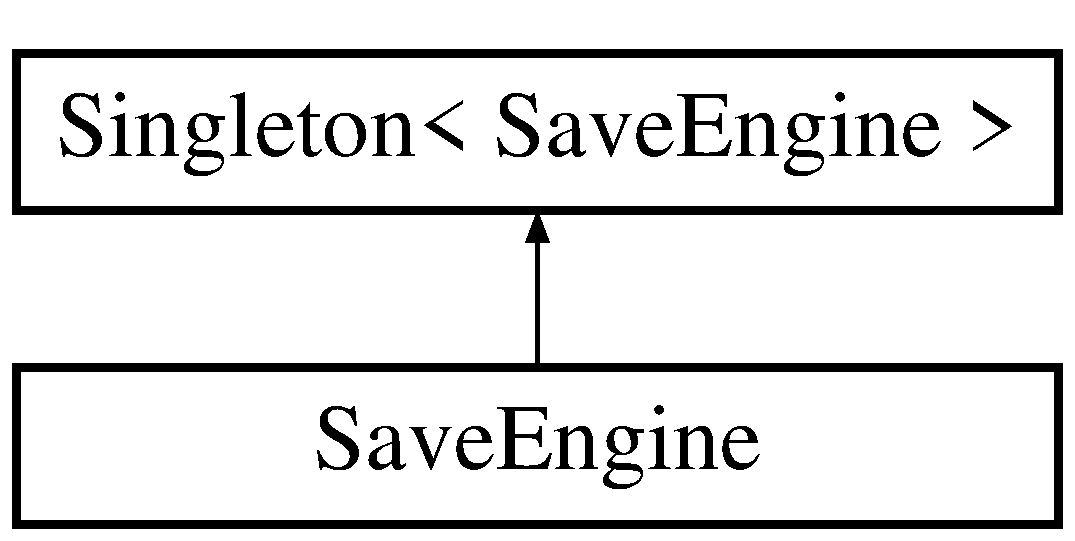
\includegraphics[height=2.000000cm]{class_save_engine}
\end{center}
\end{figure}
\subsection*{Public Member Functions}
\begin{DoxyCompactItemize}
\item 
void \mbox{\hyperlink{class_save_engine_aa1fc764f73e31736440014553f49ec1d}{Register\+Save\+Class$<$ T $>$}} (T this\+Class)
\item 
void \mbox{\hyperlink{class_save_engine_a39f4a03af6103bc9f327ba434c7d33a1}{Save\+Game}} ()
\end{DoxyCompactItemize}
\subsection*{Public Attributes}
\begin{DoxyCompactItemize}
\item 
\mbox{\Hypertarget{class_save_engine_aa7b27b629384a9039a8a1fce7d2cdd2c}\label{class_save_engine_aa7b27b629384a9039a8a1fce7d2cdd2c}} 
string \mbox{\hyperlink{class_save_engine_aa7b27b629384a9039a8a1fce7d2cdd2c}{Save\+Name}}
\begin{DoxyCompactList}\small\item\em Name for your save file. \end{DoxyCompactList}\end{DoxyCompactItemize}
\subsection*{Protected Member Functions}
\begin{DoxyCompactItemize}
\item 
\mbox{\Hypertarget{class_save_engine_a7acdd7c43a03ed9d92be36626e11d231}\label{class_save_engine_a7acdd7c43a03ed9d92be36626e11d231}} 
override void {\bfseries Init} ()
\end{DoxyCompactItemize}


\subsection{Detailed Description}
Save engine core function. 

\mbox{\hyperlink{class_save_engine}{Save\+Engine}} class
\begin{DoxyItemize}
\item Create empty Game\+Object and add Save\+Engine.\+cs on property. 
\end{DoxyItemize}

\subsection{Member Function Documentation}
\mbox{\Hypertarget{class_save_engine_aa1fc764f73e31736440014553f49ec1d}\label{class_save_engine_aa1fc764f73e31736440014553f49ec1d}} 
\index{Save\+Engine@{Save\+Engine}!Register\+Save\+Class$<$ T $>$@{Register\+Save\+Class$<$ T $>$}}
\index{Register\+Save\+Class$<$ T $>$@{Register\+Save\+Class$<$ T $>$}!Save\+Engine@{Save\+Engine}}
\subsubsection{\texorpdfstring{Register\+Save\+Class$<$ T $>$()}{RegisterSaveClass< T >()}}
{\footnotesize\ttfamily void Save\+Engine.\+Register\+Save\+Class$<$ T $>$ (\begin{DoxyParamCaption}\item[{T}]{this\+Class }\end{DoxyParamCaption})}


\begin{DoxyItemize}
\item Register which property or field that must be save.
\item This function also load data from saved file.
\end{DoxyItemize}

usage\+: \begin{quote}
Save\+Engine.\+Instance.\+Register\+Save\+Class(this);\end{quote}
\mbox{\Hypertarget{class_save_engine_a39f4a03af6103bc9f327ba434c7d33a1}\label{class_save_engine_a39f4a03af6103bc9f327ba434c7d33a1}} 
\index{Save\+Engine@{Save\+Engine}!Save\+Game@{Save\+Game}}
\index{Save\+Game@{Save\+Game}!Save\+Engine@{Save\+Engine}}
\subsubsection{\texorpdfstring{Save\+Game()}{SaveGame()}}
{\footnotesize\ttfamily void Save\+Engine.\+Save\+Game (\begin{DoxyParamCaption}{ }\end{DoxyParamCaption})}


\begin{DoxyItemize}
\item This function for save game data
\item Data is from all registered properties and field (see \mbox{\hyperlink{class_save_manager}{Save\+Manager}})
\end{DoxyItemize}

usage\+: \begin{quote}
Save\+Engine.\+Instance.\+Save\+Game();\end{quote}


The documentation for this class was generated from the following file\+:\begin{DoxyCompactItemize}
\item 
Save\+Engine.\+cs\end{DoxyCompactItemize}

\hypertarget{class_save_manager}{}\section{Save\+Manager Class Reference}
\label{class_save_manager}\index{Save\+Manager@{Save\+Manager}}


attribute for marking property or field that you want to save .  


Inheritance diagram for Save\+Manager\+:\begin{figure}[H]
\begin{center}
\leavevmode
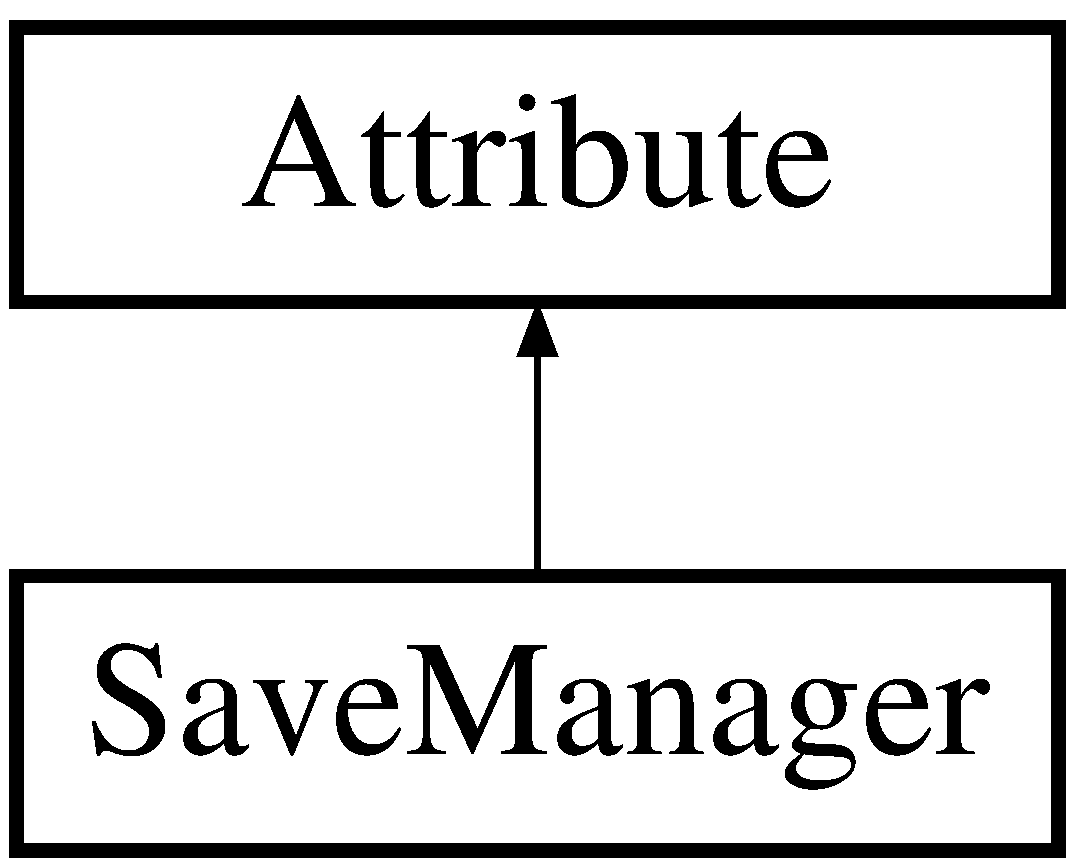
\includegraphics[height=2.000000cm]{class_save_manager}
\end{center}
\end{figure}
\subsection*{Properties}
\begin{DoxyCompactItemize}
\item 
\mbox{\Hypertarget{class_save_manager_a43e7c0b8ede3057239a0f76122759550}\label{class_save_manager_a43e7c0b8ede3057239a0f76122759550}} 
string {\bfseries Name\+Save}\hspace{0.3cm}{\ttfamily  \mbox{[}get, set\mbox{]}}
\end{DoxyCompactItemize}


\subsection{Detailed Description}
attribute for marking property or field that you want to save . 


\begin{DoxyItemize}
\item Attribute for marking and give name public properties or field that you want to save.
\item Name is for field on save database
\item Currently only int, float, string, and double data types

usage\+: \begin{quote}
\mbox{[}\mbox{\hyperlink{class_save_manager}{Save\+Manager}}(Name\+Save = \char`\"{}\+Status\char`\"{})\mbox{]} public int Status;\end{quote}

\end{DoxyItemize}

The documentation for this class was generated from the following file\+:\begin{DoxyCompactItemize}
\item 
Savemanager.\+cs\end{DoxyCompactItemize}

%--- End generated contents ---

% Index
\backmatter
\newpage
\phantomsection
\clearemptydoublepage
\addcontentsline{toc}{chapter}{Index}
\printindex

\end{document}
